% sage_latex_guidelines.tex V1.20, 14 January 2017

\documentclass[Afour,sageh,times]{sagej}

\usepackage{moreverb,url}

\usepackage[breaklinks=true, bookmarks=true, bookmarksdepth=3, colorlinks,bookmarksopen,bookmarksnumbered,citecolor=red,urlcolor=red]{hyperref}

\usepackage[T1]{fontenc}
% T1 fonts will be used to generate the final print and online PDFs,
% so please use T1 fonts in your manuscript whenever possible.
% Other font encondings may result in incorrect characters.
%
\usepackage{graphicx}

% Used for displaying a sample figure. If possible, figure files should
% be included in EPS format.
%
% If you use the hyperref package, please uncomment the following two lines
% to display URLs in blue roman font according to Springer's eBook style:
%\usepackage{color}
%\renewcommand\UrlFont{\color{blue}\rmfamily}
%\urlstyle{rm}
%
\usepackage[backend=biber]{biblatex}
%% Declare bibliography sources (one \addbibresource command per source)
\addbibresource{references.bib}

%%
\usepackage{listings}
%% auto break lines
\lstset{
  breaklines=true,
  basicstyle=\fontsize{8}{9}\selectfont\ttfamily,
}
\usepackage{xcolor} % For coloring text
\newcommand{\pc}[1]{\textcolor{red}{Pieter: #1}}
\newcommand{\rt}[1]{\textcolor{blue}{RT: #1}}
\newcommand{\jr}[1]{\textcolor{orange}{JR: #1}}
\usepackage{svg}
\usepackage{sepfootnotes}
\usepackage{amsmath}
\usepackage{stmaryrd}
\usepackage{amsfonts}
\usepackage{amssymb}
\usepackage{algorithm}
\usepackage{algorithmic}
\usepackage{subfig}
\usepackage{placeins}
\usepackage{nameref}
\usepackage{enumitem}
\usepackage{multirow}
\usepackage{amsthm}
%\usepackage[mathlines, switch]{lineno}

\newtheorem{definition}{Definition}

\newif\ifanonymous
%\anonymoustrue

\setlength{\textfloatsep}{10pt plus 1.0pt minus 2.0pt}
\setlength{\floatsep}{8pt plus 1.0pt minus 2.0pt}
\setlength{\intextsep}{8pt plus 1.0pt minus 2.0pt}

\renewcommand{\algorithmicrequire}{\textbf{Input:}}
\renewcommand{\algorithmicensure}{\textbf{Output:}}

\newcommand{\mIRI}{\ensuremath{\mathit{IRI}}}
\newcommand{\miri}{\ensuremath{\mathit{iri}}}

\newcommand\BibTeX{{\rmfamily B\kern-.05em \textsc{i\kern-.025em b}\kern-.08em
T\kern-.1667em\lower.7ex\hbox{E}\kern-.125emX}}

\def\volumeyear{2016}

\usepackage{csquotes}
% Packages
\usepackage[dvipsnames,svgnames]{xcolor} % text color
\usepackage[normalem]{ulem} % wavy underlines

% Comments
\newcommand{\todo}[1]{\noindent\textcolor{red}{{\bf \{TODO}: #1{\bf \}}}}
\newcommand{\TODO}[1]{\todo{#1}}
\newcommand{\citeneeded}{\textcolor{red}{{\bf [?!]}}}
\newenvironment{draft}{\color{gray}}{\color{black}}

% Reviewers
\newcommand\rv[1]{{\color{RubineRed}\textbf{RV}: #1}}

% Annotations
\makeatletter
\font\uwavefont=lasyb10 scaled 700
\def\spelling{\bgroup\markoverwith{\lower3.5\p@\hbox{\uwavefont\textcolor{Red}{\char58}}}\ULon}
\def\grammar{\bgroup\markoverwith{\lower3.5\p@\hbox{\uwavefont\textcolor{LimeGreen}{\char58}}}\ULon}
\def\phrasing{\bgroup\markoverwith{\lower3.5\p@\hbox{\uwavefont\textcolor{RoyalBlue}{\char58}}}\ULon}
\let\rephrase\phrasing
\newcommand\remove{\bgroup\markoverwith{\textcolor{red}{\rule[0.5ex]{2pt}{0.4pt}}}\ULon}
\newcommand\insertion{\bgroup\markoverwith{\textcolor{Green}{\rule[-0.5ex]{2pt}{0.6pt}}}\ULon}
\makeatother


\begin{document}
%\linenumbers
\runninghead{Traveling with a Map: Reducing the Search Space of Link Traversal Queries Using RDF Shapes}

\title{Traveling with a Map: Reducing the Search Space of Link Traversal Queries Using RDF Shapes}
\ifanonymous
      \author{Anonymous}
    \else
      \author{Bryan-Elliott Tam\affilnum{1}, Joachim Van Herwegen\affilnum{1}, Pieter Colpaert\affilnum{1}, Ruben Verborgh\affilnum{1} and Ruben Taelman\affilnum{1}}

      \affiliation{\affilnum{1}Department of Electronics and Information Systems, Ghent University – imec}

      \corrauth{Bryan-Elliott Tam}

      \email{bryanelliott.tam@ugent.be}
   \fi 


\begin{abstract}
% Context  
The centralization of web information raises legal and ethical concerns, particularly in social, healthcare and education applications.
% Need  
Decentralized architectures, offer a promising alternative, but efficient query processing remains a challenge.  
Link Traversal Query Processing (LTQP) enables querying across decentralized networks but suffers from long execution times and high data transfer due to excessive HTTP requests.  
% Task  
We propose a shape-based pruning approach that relies on \emph{shape indexes} and a \emph{query-shape subsumption} algorithm to reduce the search space and consequently, the number of HTTP requests.
% Object  
We formalize this method as a link pruning mechanism for LTQP and evaluate its impact on social media queries using the SolidBench benchmark.  
% Findings  
Our results show that shape-based pruning improves query execution time and reduces network usage up to 7 times compared to the state of the art, in exchange of a minor increase in the number of triples per shape-index instance.
% Conclusion  
This work demonstrates the potential of shape-based metadata for optimizing LTQP queries in decentralized knowledge graphs, going beyond its traditional use on data validation.

\keywords{Linked Data,
Link Traversal Query Processing,
RDF data shapes,
Decentralization,
Data summarization
}

\end{abstract}


\keywords{Linked Data,
Link Traversal Query Processing,
RDF data shapes,
Decentralization,
Data summarization
}

\maketitle

\section{Introduction}
\sepfootnotecontent{sf:webID}{
    \url{https://www.w3.org/wiki/WebID}
}
\sepfootnotecontent{sf:dataSovereignty}{
    \url{https://digital-strategy.ec.europa.eu/en/policies/strategy-data}
}

Data sovereignty seeks to establish a more just definition of personal data ownership in terms of data usage and storage.
It can be defined as ``the self-determination of individuals and organizations concerning to the use of their data''~\cite{verstraete2022solid},
which in practice can be interpreted as the power to choose where one's data is stored and who has access to it~\cite{verstraete2022solid}.
Multiple studies have denoted problems of ownership, democracy, reinforcement of inequality, and antagonism between users and owners of web social applications~\cite{Terranova2000FreeLP, Curran2016ch1, Sevignani2013, 9663788}.
Several authors consider decentralizing web data an insufficient solution~\cite{9663788, Curran2016ch1}; yet, it is an integral component of initiatives focused on data sovereignty,
which necessitates technical research.
Linked Data enables the creation of Decentralized Knowledge Graphs (DKGs) through the use of dereferencable IRIs.
These IRIs allow access to additional Knowledge Graphs (KGs) containing information relevant to what an IRI identifies.
For example, a WebID~\sepfootnote{sf:webID} represents a user, dereferencing it can provide the name of the user, among other information, without having to store the information locally.
Despite these benefits, most SPARQL query processing occurs in centralized setups, partly because there is a better understanding of how to optimize queries in centralized environments.

Link Traversal Query Processing (LTQP)~\cite{Hartig2012} is a query paradigm designed for querying unindexed, decentralized environments by leveraging the descriptive power of IRI dereferencing.
LTQP involves recursively dereferencing IRIs discovered in a query engine's internal triple store during query execution to expand its base of information.
The main difficulty of LTQP is the large domain of exploration, which leads to a high number of HTTP requests as demonstrated by \citeauthor{hartig2016walking}~\cite{hartig2016walking}.
From another perspective, and without contradicting \citeauthor{hartig2016walking}~\cite{hartig2016walking}, \citeauthor{Taelman2023}~\cite{Taelman2023} have demonstrated that in Decentralized Environments with Structural Properties (DESPs), it is possible to attain query completeness for various types of practical queries within acceptable execution times for the context of social media applications~\cite{nielsen1993response}.
%Moreover, they showed that query planning could significantly influence the execution time.
Structural properties ensure data discoverability, which in turn helps guarantee result completeness.
In practice, DESPs emerge in various contexts, such as social networks~\cite{Taelman2023} and the publication of sensor data~\cite{tam_iswc_traversalsensortree_2024}, among others.
%Concrete DESPs has been shown to be beneficial for datasets following the Solid protocol~\cite{Taelman2023} and the TREE specification~\cite{tam_iswc_traversalsensortree_2024}.
The work of \citeauthor{Taelman2023}~\cite{Taelman2023} indicates that there are multiple optimizations possible in LTQP in the context of decentralized environments with structural properties as opposed to the
more pessimist conclusion of the work of \citeauthor{hartig2016walking}~\cite{hartig2016walking} in the context of Open Linked Data without structural properties.

In general, the Web lacks a structure that query engines can exploit for optimization.  
This is because any document can be published anywhere, with no standard index or trust mechanism to guide discovery.  
However, within specific \emph{subwebs}, defined as subsections of the Web controlled by particular data providers, implicit or explicit data structures may emerge, which query engines can leverage.
In this work, we build on a dataset summarization approach for decentralized environments called a \emph{shape index}~\cite{tam2024opportunitiesshapebasedoptimizationlink} to enable link pruning within LTQP.  
This method maps the content of a decentralized dataset using RDF data shapes.  
This paper presents our link pruning approach using shape indexes and experimental results using a synthetic benchmark used in LTQP research.

\iffalse
This paper is organized as follows: first, we discuss the \hyperref[sec:related_work]{related work} and present \hyperref[sec:preliminaries]{preliminaries}.
We then describe our \hyperref[sec:approach]{approach}, we then introduce the \hyperref[sec:problem_statement]{problem statement}, followed by the \hyperref[sec:experiment]{experimental setup} and the \hyperref[sec:result]{discussion of results}.
Finally, we conclude the article.
\fi
\section{Related Work}

LTQP is a SPARQL querying paradigm that answers queries by exploring the web using the follow-your-nose principle~\cite{hartig2016walking}.
The main challenge of LTQP is the web's open-ended nature leading to large search space.
Completeness in LTQP is defined by the traversal of a well-defined set of links~\cite{Hartig2012}.
The first method employed to define this set was the reachability criteria~\cite{Hartig2012}, which are boolean functions that determine whether a link should be dereferenced.
Building on this, the theoretical query language LDQL~\cite{hartigLDQL} was introduced, separating the traversal definition from the query definition.
Further advancements include the subweb specifications language (SWSL)~\cite{Bogaerts2021LinkTW}, which allows data providers to define how their DKG should be traversed.
These contributions are centered on guiding the engine in selecting links to follow (discovery process).
However, they do not explicitly address mechanisms for restricting certain links (pruning process).
Link pruning can be very useful to reduce the search domain of queries when information about the data model of DKG is found.

RDF data shapes are used for validating, describing, and communicating data structures, as well as generating data and driving user interfaces~\cite{Gayo2018a,Gayo2018}.
The two main RDF data shape formalisms are SHACL and ShEx.
Both describe RDF data but differ in focus: ShEx emphasizes graph structure, while SHACL targets constraints.
For common use cases, they are equally expressive and interchangeable~\cite{Gayo2018c}.
Automatic generation of RDF data shapes based on knowledge graph (KG)~\cite{fernandez2023extracting} and shape-based integration of data~\cite{LabraGayo2023} are also topics that have been studied and can support shape-based summary approaches.
Shape Trees~\cite{shapetreesShapeTrees} is an index structure for validating and organizing decentralized knowledge graphs (DKG).
However, Shape Trees have not been used for query optimization, and the way they are formalized makes this use difficult.
RDF data shapes have also been used in the litterature for querying of centralized KG~\cite{kashif2021}.

Source selection is a crucial challenge in decentralized querying.
Approaches like SPARQL \texttt{SERVICE} clauses, service descriptions, basic statistics on triple counts, and histogram methods have been studied~\cite{hose2012towards, Harth2010}.
However, most of those source selection methods face the limitation of assuming a small number of data sources~\cite{Harth2010}, leaving their suitability for LTQP uncertain.
Bloom filters~\cite{dia2018fast} is also a mecanism that has with success for federated DKG, however in the context of LTQP it has been show that bloom filters have little effect on performances~\cite{Hanski2024}
Schemas-based indexing~\cite{Stuckenschmidt2004} using ontologies has also been explored for source selection of SPARQL queries,
however the proposed approach is sensible to the high reuse of vocabulary terms in RDF~\cite{Harth2010}.
\section{Preliminaries}\label{sec:preliminaries}

\subsection{RDF knowledge graphs and SPARQL queries}

Our work focuses on the union of conjunctive queries over RDF knowledge graphs~(KG) using the SPARQL query language~\cite{w3SPARQLQuery}.
The core components of KGs and SPARQL queries are respectively the triples and the triple patterns as deined in Definition~\ref{def:triple} and ~\ref{def:triplePattern}.

\begin{definition}[Triple]\label{def:triple}
    RDF triple $t = (s,p,o)$ are tuples formed with three terms. A subject where $s \in\mathcal{I} \cup \mathcal{B}$, a predicate $p \in \mathcal{I}$ and an object $o \in \mathcal{I} \cup \mathcal{L} \cup \mathcal{B}$.
    Where $\mathcal{I}$, $\mathcal{B}$, $\mathcal{L}$,  are respectively the set of every possible IRI, blank node, literal.
\end{definition}

\begin{definition}[Triple pattern]\label{def:triplePattern}
    Triple patterns $tp = (s_{tp}, p_{tp}, o_{tp})$ are similar to triples, where $s_{tp} \in \mathcal{I} \cup \mathcal{B} \cup \mathcal{V}$,
    $p_{tp} \in \mathcal{I} \cup \mathcal{V}$ and an object term  $o_{tp} \in \mathcal{I} \cup \mathcal{L} \cup \mathcal{V} \cup \mathcal{B}$.
    Where $\mathcal{V}$ is the set of every possible variable.
    %A triple pattern returns a solution sequence with solution mappings a single or multiple $tp$ forms a Basic Graph Pattern (BGP).
\end{definition}

We also define two access functions to get respectively the subject and object term of a triple pattern or a triple while ignoring literals,
$ S: tp \rightarrow \mathcal{I} \cup \mathcal{B} \cup \mathcal{V}$ and $O: tp \rightarrow \mathcal{I} \cup \mathcal{B} \cup \mathcal{V}$.
We denote $[\![ Q ]\!]^{G}$ as the evaluation of a query $Q$ over a KG $G$~\cite{Angles2008}.

\subsection{Reachability Criteria}

LTQP defines completeness on the traversal of links instead of the query results~\cite{Hartig2012}.
To formalize the completeness of queries, a link discrimination formalism has been developed called \emph{Reachability criteria}~\cite{Hartig2012}.
Reachability criteria are boolean functions ($c_i$) restricting the dereferencing of links from the internal data source of the query engine.
They take as parameters an RDF triple $t$ from an internal triple store, a dereferenceable IRI $iri$ from $t$, and a union of conjective queries $Q$~\cite{Hartig2012}.
If $c_i$ returns $true$, the query engine must dereference $iri$.
More formally
\begin{equation}\label{eq:reachabilityCriteria}
c_i(t, iri, Q) \rightarrow \{\mathrm{true}, \mathrm{false}\}
\end{equation}

\subsection{Decentralized Knowledge Graphs and subweb}\label{sec:dkg}

We define a DKG as a KG $G$ materialized in a network of resources $R$.
A resource $r_i \in R$ is map to a KG $g_i \subseteq G$, which is a set of triples~\cite{w3ConceptsAbstract}.
We denote this mapping $r_i \mapsto_{g} g_i$.
A resource is mapped and exposed by an IRI $iri_i$ denoted by $iri_i \mapsto_{iri} r_i$.
The network forms a graph where the resources $r_i$ are the nodes and the $iri_j \in g_i$ are directed edges starting from $r_i$ to $r_j$.
$G$ is formed by the union of all the $g \in \text{dom}(R)$.%, such that $G = \bigcup_{i=1}^{n}g_i$ given $n$ resources in the network.
A subweb is a (sub)DKG defined by a set of IRIs controlled by a data provider, which can offer a structure that aids query engine optimization.
\section{Approach}

\sepfootnotecontent{sf:shapeIndexURL}{
   \ifanonymous
      \url{https://anonymous.4open.science/w/shape-index-specification-707E}
   \else
      \url{https://constraintautomaton.github.io/shape-index-specification/}
   \fi
}

\sepfootnotecontent{sf:subwebsep}{
   We assume an implicit conversion between the subweb specification and the formalization of reachability criteria.
   Space constraints prevent us from detailing the conversion.
}

\sepfootnotecontent{sf:ssf_project}{
   The paper \citetitle{delva2023} additional material also proposes a script to convert SCHACL shapes into SPARQL queries.
   \url{https://github.com/MaximeJakubowski/ssf_project}
}

\subsection{Structured Linked Data Environments and Completeness}\label{sec:slde}
From a holistic perspective, the web does not have a structure exploitable by query engines for optimization.
On the web, any document can be published at any location, and there is no index or trust mechanism to guide source selection.
From a perspective where the web is divided into small subsections controlled by data providers, data publishers can implicitly or explicitly organize their data  
in a way that query engines could exploit its organization for optimization.
The concept of \emph{structural assumptions}~\cite{Taelman2023} has been theorized to optimize queries by exploiting the local structure of decentralized RDF datasets.
These assumptions rely on data providers guaranteeing the completeness of results for their statements within a specific set of resources in an IRI domain~\cite{Bogaerts2021LinkTW}.
Structural assumptions have been shown to reduce the query execution time of multiple queries to the extent that the bottleneck of specific queries is not the number of HTTP requests but the suboptimal query plan~\cite{Taelman2023, eschauzier_quweda_linkqueue_2023}.
Structural assumptions define completeness of traversal of SLDE in the same paradigm as reachability criteria~\cite{Hartig2012}.
We propose to put our focus on the completeness of results when considering that the completeness of traversal has been fixed.
Placing our focus on results allows us to investigate ways to optimize the search space of link traversal queries.
Our approach consists of defining more restricting reachability criteria~\cite{Hartig2012} while ensuring the same completeness of results as with less restricting criteria.


We formalize our approach as follows.
A query is executed over a DKG $G$ formed by the union of all the $g \in r$ in a network $R$.
The query engine has to build a KG $G^{\prime}$ in its internal data store from the  $g \in r$ by dereferencing resources in $R$ such that
$G^{\prime} \subseteq G$ to answer its query.
We are trying to solve an optimization problem where another query engine builds a KG
$G^{\prime\prime} \subseteq G^{\prime}$
smaller than the one produced with a specific traversal completeness policy
by defining a reachability criterion $C_{mr}$.
Because we focus on maintaining the same results completeness, then when using $C_{mr}$ the following equation must hold

\begin{equation}\label{eq:evalQueryStructuralAssumption}
   [\![ Q ]\!]^{G^{\prime\prime}} = [\![ Q ]\!]^{G^{\prime}}
\end{equation}
for any network $R$.

Because the $g \in G^{\prime}$ can only be acquired from the dereferencing of resources $r \in R$, a smaller $G^\prime$ implies that a lesser number of HTTP requests has been performed to answer a query.
Naturally, query execution is faster with a smaller KG instance.
Additionally, HTTP requests can be slow and unpredictable~\cite{hartig2016walking}, making them a significant factor in overall query execution time. 
Thus, the benefit of reducing the number of HTTP request is twofold.

To define less selective reachabilities to produce $G^{\prime\prime}$, we propose extending the reachability criteria by formalizing a chain of criteria in a concept called \emph{composite reachability criteria}.
In this form, a reachability criterion $cp_i$ is said to \emph{prune} links, and $cd_i$ is said to \emph{discover} links.
A reachability $cp_i \in C$ should act upon all the links that have yet to be dereferenced as well as on the incoming links.
Equation~\ref{eq:cReachabilityCriteria} formalizes a composite reachability criterion $C$ with $nd$ discovery criteria and $np$ pruning criteria.

\begin{equation}\label{eq:cReachabilityCriteria}
   C(t, i_d, B) = \bigvee_{cd \in Cd} cd(t, i_d, B) \mathrel{\land} \bigwedge_{cp \in Cp} \, cp(t, i_d, B)
\end{equation}
where $Cd$ is the set of every $cd_i(t, i_d, B)$ and $Cp$ the set of every $cp_i(t, i_d, B)$ used by the engine.
\iffalse
Maybe refer to the link queue here in a footnote.
\fi

\iffalse
In the context of the World Wide Web (WWW), defining completeness based on results is not possible because it necessitate the acquisition of the whole web.
However, in the context of a decentralized dataset with structural properties and associated structural assumptions,
the traversal completeness of those datasets is defined outside of the query engine and thus can serve as a 
stable comparison concept regardless of the traversal policy of the engine.
Hence, for each dataset with structural properties, it is possible to compute a theoretical result completeness.
If we suppose a finite network of connected datasets that are discoverable with a specified reachability criterion such as \texttt{cmatch},
Then, it is possible to establish the completeness of the subset of the query targeting information in the network.



Furthermore, having a stable traversal completeness we can create a theorical results completeness metric, by considering the descentralized dataset as a centralized one that is the union 
of all the knowledge graph inside the ressources of the dataset $GD = \bigcup\limits_{i}^{n} g\in r_i$ given $n$ ressource $r$.
This, metric 

\begin{equation}\label{eq:metricResult}
   [\![ Q ]\!]^{G^{\prime}} = [\![ Q ]\!]^{G}
\end{equation}

\fi 



\iffalse
While BQPs are syntactic objects, we shall use them as a represen-
tation of Linked Data queries which have a certain semantics. In the
remainder of this section we define this semantics. Due to the open-
ness and distributed nature of Webs such as the WWW we cannot
guarantee query results that are complete w.r.t. all Linked Data on
a Web. Nonetheless, we aim to provide a well-defined semantics.
Consequently, we have to limit our understanding of completeness.
However, instead of restricting ourselves to data from a fixed set
of sources selected or discovered beforehand, we introduce an ap-
proach that allows a query to make use of previously unknown data
and sources. Our definition of query semantics is based on a two-
phase approach: First, we define the part of a Web of Linked Data
that is reached by traversing links using the identifiers in a query
as a starting point. Then, we formalize the result of such a query
as the set of all valuations that map the query to a subset of all
data in the reachable part of the Web. Notice, while this two-phase
approach provides for a straightforward definition of the query se-
mantics in our model, it does not correspond to the actual query
execution strategy of integrating the traversal of data links into the
query execution process as illustrated in Section 2.

The analysis
of this implementation approach is particularly interesting because
this approach trades completeness of query results for the guarantee
that all query executions terminate as we shall see.


Hartig2012
\fi


\subsection{Shape Index}

We propose using a decentralized dataset summary method, called the shape index~\cite{tam2024opportunitiesshapebasedoptimizationlink}, as the support mechanism for our pruning reachability criterion.
This method involves mapping the content of a decentralized dataset using RDF data shapes.
The intuition behind this approach is that rendering explicit RDF schemas is relatively inexpensive for data providers when publishing decentralized datasets.
Although RDF does not enforce schemas on its data, the nature of the usually modeled objects and the formalism often results in implicit schemas~\cite{Neumann2011CharacteristicSA}.
Additionally, the cost of making these schemas explicit should be evaluated in the context of the data's intended usage.
First, mapping and documenting decentralized data improves its discoverability, which is a common objective when publishing RDF data.
Second, embedding this information within datasets facilitates client-side query engine processing, potentially reducing reliance on costly SPARQL endpoints~\cite{aranda2013}.
Since the web is a highly dynamic environment where data providers require flexibility, shape indexes support open shapes as mapping keys.
For example, a data provider might expose personal data such as movie recommendations, bookmark metadata, and friend lists.
The provider might use open shapes for movie recommendation data because they are less structured and employ closed shapes for bookmark and friend list data.

A shape index 
\begin{equation}\label{eq:shapeIndex}
   SI = \{s_1 \mapsto IRI_1, s_2 \mapsto IRI_2 \cdots, s_n \mapsto IRI_n\}
\end{equation}
, is a mapping between RDF data shapes and a set of IRI given $n$ entries.
The domain of a shape index is defined by $D = \bigcup_{i=1}^{n} \bigcup_{iri \in IRI_i} iri$.
A shape index \emph{must} map every resource in $D$.
We denote a shape index as \emph{complete} when every shape $s_i \in SI$ is closed and \emph{incomplete} otherwise.
A mapping between a shape and a set of IRI has implications in the distribution of the data in $D$.
When a shape $s$ is mapped to an $IRI$ then the KG $G = \{g | g \in r, iri \mapsto r \land iri \in IRI\}$ satisfy $s$.
Given that the shape mapping a set of IRI is close, then every set of triple in the resource associated with $D$ respecting the shape must be in a resource mapped to an $iri \in IRI$.
A draft web specification of the shape index is also available online.~\sepfootnote{sf:shapeIndexURL}

\subsection{Online Source Selection in Shape Index Documented Datasets}

A decentralized dataset exposing a shape index provides a query engine with the opportunity to reduce its search domain by evaluating which resources are query-relevant.
The shape descriptions and constraints on the distribution of the data allow the query engine, 
within a domain $D$ of a shape index $SI$ to determine a priori before traversing $D$ which subdomain $d \subseteq D$ contains data that is query-relevant.
To formalize our approach, we use the concept of composite reachability criteria described in section~\ref{sec:slde} and of the source selectors of the subweb specification formalization~\cite{Bogaerts2021LinkTW, Taelman2023}.

We propose that a query engine with composite reachability $C_t$ at any time $t$ can query an SLDE with completeness of results.
$C_t$ is defined as such that if the engine were not to change its reachability
until $t_f$, the end of the query execution, the completeness of results,
as defined in Equation~\ref{eq:evalQueryStructuralAssumption},
will remain consistent with the results obtained using the reachability at the beginning of execution, $C_{0}$.
We propose that $C_0$ must have a discovery criteria $cd_{\text{shape index}}$ that follow links leading to shape indexes.
Let us consider that the predicate \texttt{si:shapeIndexLocation} indicates that the object of the triple is the location of the shape index 
of the dataset, thus we can define the criterion
$cd_{\text{shape index}} = \{o|\forall s \langle \text{si:shapeIndexLocation} \rangle \}$.~\sepfootnote{sf:subwebsep}
A reachability $C_{tsi_i}$ is created after dereferencing a shape index.
This reachability must accept the links $IRI_d$ that are query-relevant and prune the links $IRI_p$.
To determine $IRI_d$ and $IRI_p$ a query-shape containement ($\sqsubseteq_{qs}$) is performed.
The problem is defined in section \ref{sec:containment}.
We define 
$IRI_d = \{ \bigcup_{iri \in SI_i(s_j)} iri |  B \sqsubseteq_{qs}  s_j = \mathrm{true}, s_j \in \text{DOM}(SI_i) \}$ and 
$IRI_p = \{ \bigcup_{iri \in SI_i(s_j)} iri | B \sqsubseteq_{qs}  s_j = \mathrm{false}, s_j \in \text{DOM}(SI_i) \}$

given a shape index $SI_i$.
From those sets of links we define two new reachability criteria;
\begin{equation}
   \begin{aligned}
       cd_{si}(t, i_d, B) &= i_d \in IRI_d \\
       cp_{si}(t, i_d, B) &= i_d \notin IRI_p
   \end{aligned}
\end{equation}
the new reachability $C_{tsi_i}$ is created by taking the $Cd$ and $Cp$ of $C_{tsi - 1}$ and adding
$cd_{si}$ and $cp_{si}$ to the corresponding set. 

\subsection{Expressing RDF Data shapes into SPARQL algebra}\label{sec:shape2SPARQL}

A shape expression $e_i$ can be intuitively treated as a segment of a query~\cite{delva2023}.
A common approach for shape validation over an RDF graph is to convert shapes into SPARQL queries~\cite{labragayo2017validatingdescribinglinkeddata, Corman2019,Prestamo2023, spapeExpressionConvert}.~\sepfootnote{sf:ssf_project}

\iffalse
For our query-shape containment problem we are looking into transforming our shapes $S$ into queries $Q_s =  q_i \bowtie q_{i+1} ... \bowtie q_n$ by transforming each $e_i$ of $s$ in a $q_i$.
We are looking into creating a query $Q_s$ with the following property
\begin{equation}\label{eq:shapeSPARQL}
   G \models S \iff [\![ Q_s ]\!]^{G} =  G
\end{equation}
For every $G$.

Our definition is aimed at close shapes because we are not looking into validating data but into containment since an open shape can validate 
For any $G$ that contains at least the constraint specified by $S$, we simplify the fact that if we neglect negative statements, any query can be contained in such a shape.
The intuition behind equation~\ref{eq:shapeSPARQL} is that we are looking to produce a query that simulates the behavior of a shape.
It is natural from the definition of shape languages. It has been shown in the literature that shape constraint can be transformed into a combination of triple patterns, filter expressions, and other SPARQL fragments.
Thus, if we can establish a mapping between the constraints of $S$ in terms of query fragments, a query targeting $G$ should return $G$ if every triple of the 
$G$ respects the constraint of the shape.
\fi
We define in the following lines the transformation of a shape $S$ into a query $Q_s$ using the transformation $T(S,?x)$ and $t(e_i, ?x) = q_i$ where every 
symbol with a $?$ prefix is a variable in $\mathcal{V}$.

\iffalse
INSPIRE YOURSELF BY Corman2019 style

We might want to reference that

https://labra.weso.es/publication/2023_kg_subsets_pregel/
https://labra.weso.es/publication/2024_extracting_shapes_consolidator/

https://labra.weso.es/publication/2023_rdf_data_integration/

ssf_project Maxime

https://github.com/MaximeJakubowski/ssf_project/blob/master/ssf/sparql_conformance.py

\fi

\begin{prop}\label{prop:triplePattern}
   A shape expression $e_i = st$ given $rs^a_b = st_3$ and $p$ is the predicate from $pc_p = st_1$
   can be transformed into a query consisting of one triple pattern with an associated \texttt{GROUP BY ?x HAVING(COUNT(?o))} statement on the object of triple pattern,
   such that
   $Q_{e_i} = \beta_{?x, (|?o| \in rs^a_b)}(?x, p, ?o)$,
   where $\beta$ is a \texttt{GROUP BY ?x HAVING} clause and $|?o|$ is a \texttt{COUNT} clause. 
\end{prop}

\begin{prop}
   In a shape expression $e_i$ , $oc_f = st_2$ can be transformed into a filter expression targeting $?o$ if the constraint validates an RDF type or a literal comparison.
   This transformation takes the form $q_{i} = \sigma_{oc_f((?x, p, ?o))}(?x, p, ?o)$ where $\sigma$ represent the filter expression applid on $?o$.
   If $oc_f$ validates a shape on $?o$, then $q_i$ must be formed by joining a query derived from $e_i$ with $oc_f = \mathrm{true}$ and a query derived from the shape targeted by $oc_f$ 
   where $?o$ is the subject such that $q_{i}= (?x, p, ?o) \bowtie T(S_{oc_f},?o)$ given $S_{oc_f}$ is the shape related to $oc_f$.
\end{prop}

\begin{prop}
   In a shape expression $e_i = e_j|e_k$ the expression can be transform into the union between two queries
   $q_{i} = t(e_j, ?x) \cup t(e_k, ?x)$.
\end{prop}

\begin{prop}
   In a shape expression $e_i = st$ when $st_4 = n = \mathrm{true}$ then the query $q_i$ must be negated such that $\neg q_i$ and $\beta$ statements ignored.
\end{prop}

\begin{prop}
   A closed shape ($op = \mathrm{false}$) $S$ can be transform into $Q = t(e_1, ?x) \bowtie t(e_2, ?x) ... \bowtie t(e_{n_{ec}}, ?x)$ given $n_{ec}$ shape expressions.
\end{prop}

\begin{prop}
   A open shape $S$ ($op = \mathrm{true}$) is transform into $Q = (?x, ?p, ?o) -  (t(e_1, ?x) \bowtie  t(e_2, ?x) ... \bowtie t(e_{n_{eo}}, ?x)) $
   given $n_{eo}$ negative $e_i$ (where $n = \mathrm{true}$).
\end{prop}

\subsection{Query Shape Containment}\label{sec:containment}

We propose using query containment as a source selection mechanism.
While query containment is intuitively unsuitable for online source selection due to its NP-complete complexity~\cite{Spasi2023}, this complexity depends on the size of the queries, which are typically small.
Moreover, practical use cases can leverage polynomial time complexity algorithms~\cite{Doan2012}.
In our context, the container query (the shape) follows a tree star pattern template structure where predicates are always IRIs, and subjects and objects are always variables.
This structure can be leverage to create an algorithm with polynomial time complexity algorithms.

We consider that a query $Q$ is contained into a shape $S$ denoted $Q \sqsubseteq_{qs} S$, if a tree star pattern in $Q$ is contained in $Q_s = T(S, ?x)$ where $?x$ is the variable of the subject of the body of the shape.
For a tree star pattern to be contained, we need to consider the two parts of $Q = Q_{body} \cup Q_{\text{unions}}$.
$Q_{body}$ is the Basic Graph Pattern (BGP) of the query and $Q_{\text{unions}} = \bigcup Q_u$ are the Union Graph Patterns (UGP) where $Q_u = q_0 \cup q_1 \cup q_2 ... \cup q_n$.
A tree star pattern $Q_{starT_i}$ is contained in $Q_s$ if its segment in $Q_{body}$ is contained in $Q_s$ and that the tree star pattern is contained in at least one $q_i$ in each $Q_u$ is contained in $Q_s$.
If $Q_{starT_i}$ is not a part of an $Q_u$, then the $Q_u$ is ignored.
In our containment problem we ignore "cardinality constraint" which are translated in 
fragments of the form \texttt{GROUP BY ?x HAVING(COUNT(?o))}.
We ignore these segments because we are not attempting to identify sources that can fully answer a particular segment of a query.
Instead, we attempt to disregarding data sources that are irrelevant to the query, given the constraints imposed by the shape index.
Thus, discriminating based on cardinalities might impact query results.
Additionally, in this paper, we do not consider filter expressions.

\iffalse
While evaluating filter expressions would increase the algorithm's time complexity, it would also improve the precision of source selection.
However, ignoring them does not affect the completeness of results in our context.
Therefore, the tradeoff of including them in the resolution warrants an analysis.
\fi

% https://en.wikipedia.org/wiki/Master_theorem_(analysis_of_algorithms)
\begin{algorithm}[h]
   \caption{Determine if a tree star pattern is contained ($isContain_{T}$)}\label{alg:containmentTree}
   \begin{algorithmic}
      \REQUIRE  $Q_{star}$, $Q_{starT_i}$, $Q_s = Q_{s\text{body}} \cup Q_{s\text{unions}}$ and $MS$
      \ENSURE \TRUE $ $ or \FALSE $ $ whether the tree star is contained in the shape

      \IF{$S_{star}(Q_{star}) \in MS$}
         \RETURN \TRUE
      \ENDIF 

      \FORALL{$tp \in Q_{star}$} % O(n_star)
         \IF{\NOT $match(tp, Q_{s\text{body}})$}
            \STATE $hasOnePath \gets $ \FALSE
            \FORALL{$q_{us} \in Q_{s\text{unions}}$}
               \IF{$isContain_{T}(Q_{star}, Q_{starT_i}, q_{us}, MS)$}
                  \STATE $hasOnePath \gets $ \TRUE
               \ENDIF
            \ENDFOR
            \IF{\NOT $hasOnePath$}
               \RETURN \FALSE
            \ENDIF
         \ELSE
            %eval nested
            \IF{$O(tp) \in  S_{star}(Q_{starT_i})$}
               \IF{\NOT $isContain_{T}(Q_{star_{O(tp)}} \in Q_{starT_i}, Q_{starT_i}, Q_s, MS)$}
                  \RETURN \FALSE
               \ENDIF
            \ENDIF
            %
         \ENDIF
      \ENDFOR

      \STATE $MS \gets MS \cup S_{star}(Q_{star})$
      \RETURN \TRUE
   \end{algorithmic}
\end{algorithm}


We define the function $isContain_{T}$ defined in Algorithm~\ref{alg:containmentTree} to evaluate if a $Q_{star_i}$ is contained in $Q_s$.
The $match$ function evaluates if a triple pattern independent of the variable's names is in a query.
The algorithm is recursive, and on its first call, $Q_{star}$ must be the root of the $Q_{starT_i}$, and $MS$ must be an empty set, 
this set is used not to duplicate containment calculations.
We notice that the complexity of Algorithm~\ref{alg:containmentTree} is $O( n_o \times n_{tp}^2 \times n_{sunion}^2)$
where $n_{tp}$ is the number of triple patterns of $Q_{star_i}$, $n_{sunion}$ the number of UGP in $Q_s$ and $n_o$ the number of object term in $Q_{starT_i}$.
To solve $Q \sqsubseteq_{qs} S$, we need to consider the $n_{starT}$ tree star from the BGP with their $n_{starTu}$ segment in the UGP and $n_{starTui}$ BGP in the UGP.
This operation results in a polynomial time complexity of $O(n_o \times n_{tp}^2 \times n_{union}^2 \times n_{starT} \times n_{starTu} \times n_{starTui})$.
In the \nameref{sec:appendix} Algorithm~\ref{alg:containment} present the full resolution.

\section{Experimental Evaluation}\label{sec:experiment}

We implemented our approach using the LTQP version of the Comunica query engine~\cite{taelman_iswc_resources_comunica_2018}.
We chose Comunica due to its modularity~\cite{taelman_swj_componentsjs_2022} and its established use in several LTQP studies~\cite{Bogaerts2021LinkTW, Taelman2023, eschauzier_quweda_linkqueue_2023, Hanski2024, eschauzier_amw_rcubemetric_2024, tam2024opportunitiesshapebasedoptimizationlink}.
All implementations are open-source and are provided in the \hyperref[sec:supplementalMaterial]{supplementary material}.
Similarly to other LTQP studies, we used SolidBench~\cite{Taelman2023}, which is based on the LDBC social network benchmark~\cite{Angles2020}, to evaluate our contribution.
Furthermore, SolidBench was developed because no LTQP benchmark existed prior to its creation~\cite{hartig2018linked, Taelman2023}, and, to the best of our knowledge, no other benchmarks have been introduced since.
We created an open-source module to generate shape indexes in SolidBench, based on user-provided mappings between ShEx shapes and data model objects.
The shape-annotated portion of the data model includes posts, comments on posts, user profiles, user settings, varia data (unstructured data), cities, and likes.
The datasets are Solid Pods~\cite{sambra_solid_2016, dedecker2022s}.
In this paper, we consider a Solid Pod as a web-based file system that follows the LDP specification~\cite{w3LinkedData}.
Each Solid Pod, alongside contains its data, a shape index and separate resources for each shape definition.
Some shapes are nested within others. 
For example, user profiles are associated with cities, and comments are associated with posts.
Depending on the pod instance, certain data model objects are materialized in a single file, while others are distributed across multiple files.
The benchmark provides queries that simulate typical read actions in social media use cases, such as retrieving replies to posts or identifying users connected to a given user. 
Queries may range from being highly selective with small result sets to broad with larger result sets, and in some cases can also be characterized as data-model selective.
The datasets contained approximately 4,200,000 triples and 1,528 subwebs, which, in this context, are Solid Pods.
The shape indexes contain 13 triples each, while the largest shapes have up to 150 triples. 
This can be considered insignificant, particularly because the number of triples does not scale with the size of the subwebs.
The entire data model and query templates are available in the \hyperref[sec:supplementalMaterial]{supplementary material}.

To evaluate our approach, we conducted the following experiments: 
\begin{itemize}
   \item We measured the execution time and results of our query-shape subsumption algorithm using the shapes from the study.
   \item We then compared our shape index approach to state-of-the-art Solid Pod network traversal algorithms: one leveraging the type index specification~\cite{Taelman2023}, and another using the LDP specification~\cite{Taelman2023}, in a network where each Solid Pod provides a complete shape index.~\footnote{It should be noted that the type index and shape index approach are extensions of the LDP approach.}
   \item We analyze the relationship between the number of HTTP requests and query execution time, drawing on data collected across all experiments.
\end{itemize}

Subsequently, we assessed the resilience of our approach by gradually reducing the shape index information across the network by performing the following experience:

\begin{itemize}
   \item We measured query execution time in networks where 0\%, 20\%, 50\%, and 80\% of Solid Pods expose a shape index.
   \item We measured query execution time in networks where 20\%, 50\%, and 80\% shape indexes are complete.
   \item We measured query execution time in networks having shapes that incorporate only data from the Solid Pods and shapes providing a minimal dataset description where the object constraints are always an IRI or a literal.
\end{itemize}

We conducted the experiment using queries from five different instantiations of SolidBench query templates, varying the starting pods in a random yet reproducible manner.
Experiments were repeated 50 times with a 2 minute timeout per query execution. 
They were conducted on an Ubuntu 20.04.6 LTS machine with a 2x Hexacore Intel E5645 CPU and 24GB RAM.


%https://doc.ilabt.imec.be/ilabt/virtualwall/hardware.html#virtual-wall-2

\section{Discussion of Results}\label{sec:result}

\subsubsection{Evaluation Against Other Approaches}

\begin{figure}
    \centering
    % First figure
    \begin{minipage}[t]{0.40\linewidth}
        \centering
        \includegraphics[width=\linewidth]{analysis/artefact/variation_approach/reduction_query_execution_time_raw}
    \end{minipage}
    \hspace{0.05\textwidth}
    % Second figure
    \begin{minipage}[t]{0.40\linewidth}
        \centering
        \includegraphics[width=\linewidth]{analysis/artefact/variation_approach/reduction_query_execution_time}
    \end{minipage}

    % General caption
    \caption{
    On the left is a plot showing query execution times, while the figure on the right compares the type index combined with the LDP approach against other methods.
    The ratio represents how the execution time of each method compares to that of the type index and LDP approach, a ratio greater than one indicates a slower execution time.
    The shape index approach performs similarly or better than the other methods, except in the case of S4.
    }
    \label{fig:compApproach}
\end{figure}

%\input{analysis/artefact/statistical_significance/comparaisonStateOfTheArt}


Figure~\ref{fig:compApproach} shows that the shape index approach for all query templates except S4 performs better or comparably to the state-of-the-art Solid Pod network traversal algorithm.
An analysis of statistical significance is provided in the \hyperref[sec:supplementalMaterial]{supplemental material}.
Moreover, with the shape index approach, it is possible to answer a query from the S7 template.
Queries can require as little as 13\% (S1) of the execution time (7.7 times faster) of the type index and LDP traversal algorithm.
The queries that perform the best are those in which the number of HTTP requests decreased the most, as can be inferred from the analysis of Table~\ref{tab:ratioUsefulResources}.
%Table~\ref{tab:statSignificanceStateOfTheArt} presents an analysis of the statistical significance of the query template and its relation to the ratio of HTTP requests performed.
Queries from templates D6 and D7 show no reduction because they require nearly every document in the dataset to be processed by the engine, making our approach ineffective in these cases.
We notice that queries from template S4 with the shape index performed worse in every instance, with an increase in query execution time of up to 2.80 times.
This is further illustrated in Table~\ref{tab:ratioUsefulResources}, which shows that for these queries, the type index and LDP traversal algorithm achieves a ratio of useful resources dereferenced of 100\% or 50\%, compared to only 6\% with the shape index approach.

The poor performance is due to the fact that the links acquired by the other approaches were selected based on reachability criteria that did not leverage the structural properties of the dataset, such as in the case of \texttt{Cmatch}~\cite{hartig2016walking}.
In contrast, the shape index approach always enforces the use of these properties, resulting in additional HTTP requests and increased processing time.
%It has to be highlighted that our formalization assumes that structural assumptions are always used and that the shape index, if present, will be part of the traversal, see section~\ref{sec:sourceSelection}.
However, those queries were already fast, with the type index and LDP traversal algorithm approach being executed in approximately 0.30\% of the maximum execution time allowed.
Nonetheless, these results still highlight a category of queries and networks for which our approach is not well-suited.
Those results mostly validate \textbf{H1} however the shape index approach can drastically increase the execution time when the structural properties are not used.

\subsubsection{Query-Shape Subsumption Evaluation}
The empirical evaluation of the query-shape subsumption algorithm shows that its execution time with the more detailed shapes from our experiment is negligible, with a maximum execution time of 4.655 ms (0.0039\% of the timeout).
The result tables are available in the \hyperref[sec:supplementalMaterial]{supplemental material}.
This outcome is expected, as the algorithm has polynomial time complexity, and the shapes and queries in the experiments are small and not deeply nested.
This result validated \textbf{H2}.

\iffalse
\begin{figure}[htbp]
    \centering
    % First figure
    \begin{minipage}[t]{0.40\linewidth}
        \centering
        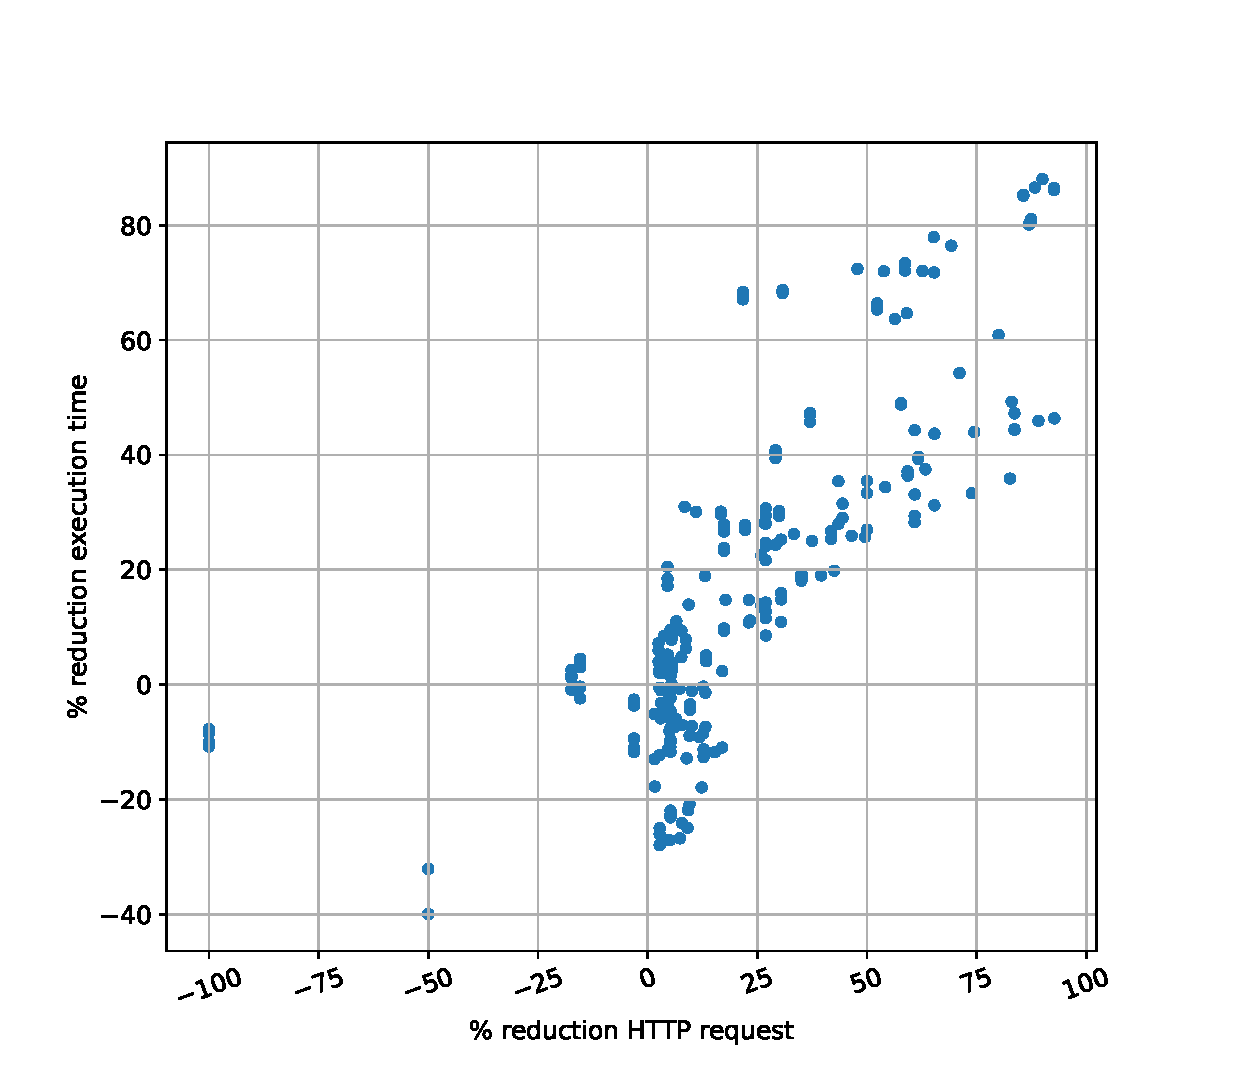
\includegraphics[width=\linewidth]{analysis/artefact/http_req_exec_time_relation/http_req_exec_time_cor_better}
        \label{fig:http_req_exec_time_cor_better}
    \end{minipage}
    \hspace{0.05\textwidth}
    % Second figure
    \begin{minipage}[t]{0.40\linewidth}
        \centering
        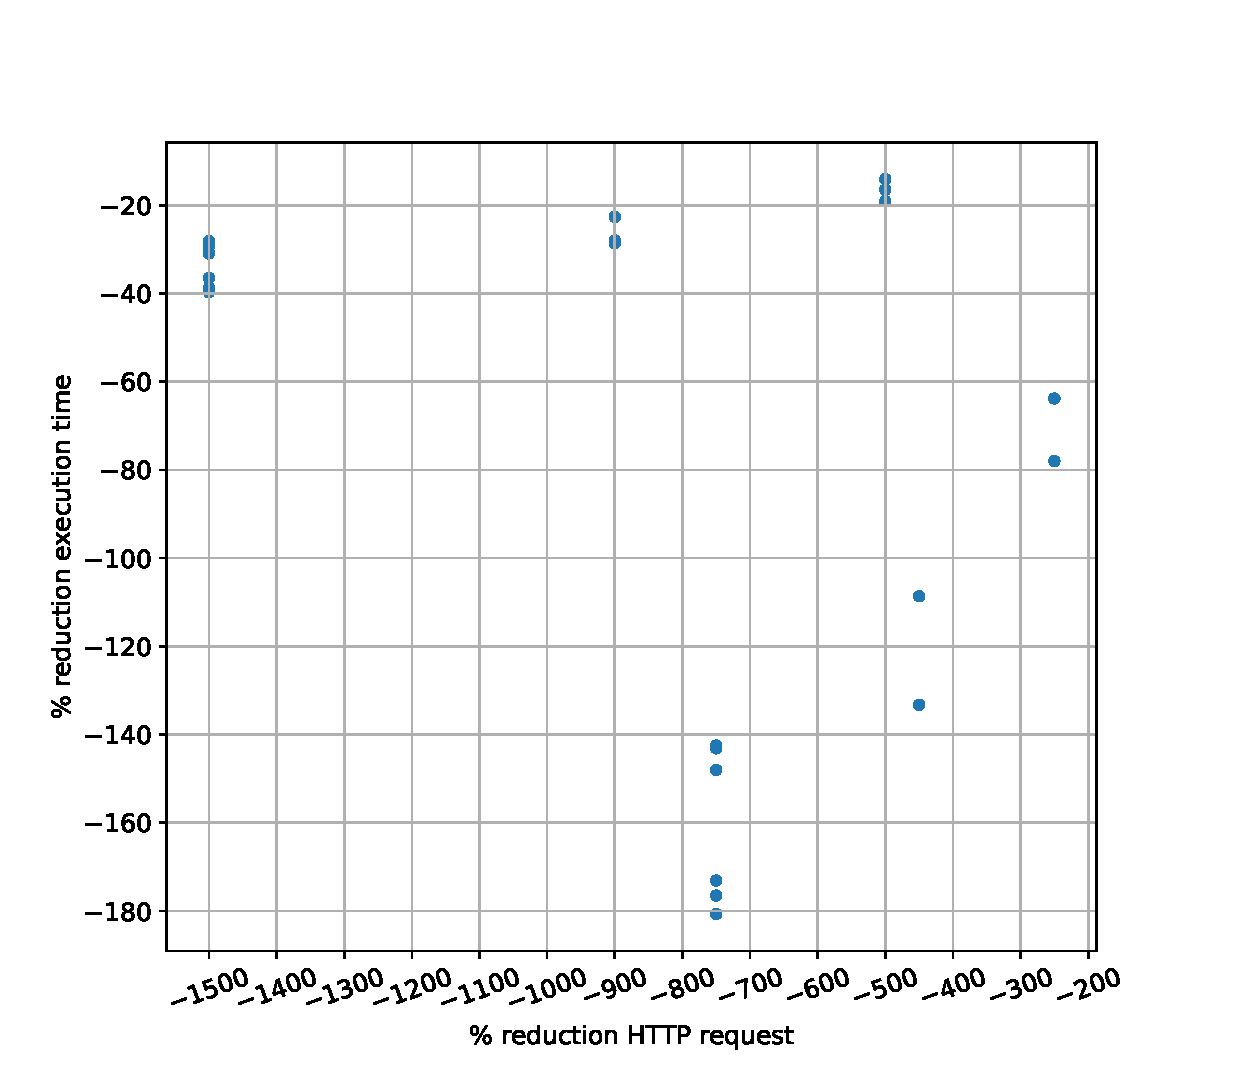
\includegraphics[width=\linewidth]{analysis/artefact/http_req_exec_time_relation/http_req_exec_time_cor_worse}
        \label{fig:http_req_exec_time_cor_worse}
    \end{minipage}

    % General caption
    \caption{
        The data show two regimes in the relation between the number of HTTP requests and the execution time, 
        we see a more linear correlation on the left figure than on the right figure.
        }
    \label{fig:http_req_exec_time_cor}
\end{figure}

\subsubsection{Relationship Between HTTP Request and Query Execution Time}

To determine the relationship between the reduction of HTTP requests and the query execution time, we evaluated their ratio using 
the data of our experiments with the Solid Pod network optimal traversal algorithm results as the baseline.
Figure~\ref{fig:http_req_exec_time_cor} present our analysis.
The relationship between HTTP request and query execution time can be divided into two regimes.
In the first regime (left figure), where the shape index approach reduces the number of HTTP requests, we notice a positive linear correlation with a
Pearson correlation coefficient (PCC) of 0.84 and a high statistical significance given $< 0.01$.
We can notice that toward the end, the curve appears to exhibit more exponential behavior.
Evaluating an $R^2$ score with an exponential best fit curve we get a score of 0.72 and 0.71 for a linear curve.
Below a ratio of approximately 0.83 of HTTP requests, the shape index approach did not guarantee a reduction in query execution time.
With this observation, the exponential behavior might be explained by the approach's overhead. 
It is possible that with a small reduction of HTTP requests, the state retention required for the pruning reachability criteria could offset the gain in the reduction of HTTP requests.
In the second regime (right figure), the shape index increases the number of HTTP requests.
We notice a weaker positive linear correlation with a PCC of 0.44 and a high statistical significance though the significance is lower than in the first regime.
The overall correlation between reducing HTTP requests and query execution time is positively linear, with a PCC of 0.56 and a high statistical significance.
The overall correlation is more linear than exponential with $R^2$ scores respectively of 0.31 and 0.24, however due to the low score it is difficult to determine the nature of the distribution.
Explaining the two regimes' behavior exhibited by the data is challenging.
A possible explanation can be the lack of samples when the shape index approach performs poorly.
However, we can also notice that the relationship between the two variables in the first regime is closer to one-on-one (slope of approximately 0.91) than in the second regime (slope of approximately 0.08), where the ratio of HTTP requests has less of an impact.
Futhermore, the number of HTTP requests increased by 16 times compared to the baseline, which initially required only 1 or 2 requests (see Table ~\ref{tab:ratioUsefulResources}). 
However, despite this increase, the engine ultimately handled a modest number of links to dereference.
This indicates that the actual impact might not be as significant as the figure suggests, particularly considering that HTTP requests are done concurrently.
Those results validate \textbf{H2} when there is a decrease in HTTP requests, however, with an increase, the results are more uncertain.
%\rt{I think this paragraph can be shorted quite a bit if you run into space issues.}
%This observation can lead us to question how complex the queries are in that regime; queries where the shape index increases vastly in the number of HTTP requests are the queries from the S4 template. 
%However, those queries were already answered quickly and consisted of only four triple patterns and a union statement (with the alternative property path). 
%Thus, it is possible that the number of HTTP requests has less of an impact because it is easier for the engine to perform the join operation upon reception of the data than when processing more complex queries.
%Additionally, those queries where already answer with 1 or 2 HTTP request with the baseline thus increase by 16 time of the number of HTTP request still leave the engine with a modest number of links to dereference.

% Analysis by query template? But we lack the space. In the appendix too...
% We can also with that explain some big gap in the plot.
\fi


\subsubsection{Evaluation of the Resilience of the approach}

The final part of the results analysis focuses on the resilience of the shape index approach.
In this analysis, we examine the impact of reducing the shape index information in the network and compare the results with a network in which all pods are exposed to detailed, complete shape indexes.
Figure~\ref{fig:adaptShapeIndex} presents three plots that illustrate the results of our evaluation of the approach's resilience.
The plot on the left shows the variation in the availability of shape indexes across the network. 
As expected, we observe that queries that performed better in Figure~\ref{fig:compApproach} tend to perform worse with reduced shape index information, while queries that performed poorly improved. 
%Queries that were unaffected by the shape index changes remain unaffected.


\begin{figure}
    \centering
    \includegraphics[width=1\linewidth]{analysis/artefact/variation_shape_index_all/plot}
    \caption{
    Shape index approaches tend to perform less effectively with limited network information and comparatively better where the baseline shape index underperforms.
    A higher ratio indicates a longer query execution time compared to a network with complete shape index information.
    However, the utility of shape index information can vary depending on the specific queries and network characteristics.
    }
    \label{fig:adaptShapeIndex}
\end{figure}


The plot in the middle shows the variation in the percentage of shape index entries using closed shapes.
The results here are more nuanced.
While there is a general trend for query evaluations with a lower percentage of closed shapes to behave similarly to the plot on the left, we also observe both performance gains for some query template and a drastic performance loss for the queries of S1 when 80\% of the shape entries are closed.
The performance gain occurs because not every entry needs to be closed to prune the query irrelevant documents.
Entries mapped to an open shape are always considered relevant because the shape translates to a query fetching the whole KG.
If the subsumption check leads to the same conclusion, then, given a closed entry, the execution will be more expensive because 
when shapes are nested, the nested shapes need to be dereferenced to solve the query-shape subsumption algorithm.
For the queries of S1, with 80\% of closed shape entries, the performance lost was due to random chance, as the discriminatory entries were provided with open shapes in multiple instances when looking at the raw data.

The right plot shows the variation in the level of detail of the shapes by reducing their detail.
Since the shapes are closed in this experiment the level of detail was varied by changing the constraint of the object terms of the shape as describe in Section~\ref{sec:experiment}.
Most queries tend to perform similarly or better, with the exception of those of S1.
Upon analyzing the output of our query subsumption algorithm, we observe that the additional information to the shape provided in our base approach does not affect the algorithm’s results.
However, in the baseline shape index experiment, the engine must dereference more shapes, potentially increasing execution time.
Queries of template S1 is the only one where the added information can discriminate multiple parts of the datasets' domain, indicating the intuitive results that, in some situations, adding more information can be beneficial.
This sensitivity of the quantity of the information in the index also helps explain the results for S1 queries in the middle plot. 
In that case, the engine still had to dereference sources from each dataset, and the information available was likely insufficient to significantly discriminate between sources.

\input{analysis/artefact/ratio_useful_resources/table_ratio_useful_ressources} 

Those results show that \textbf{H3} is rejected; reducing information is rarely detrimental for query execution, except in cases where added information is critical to determine the query relevance of sources.
Thus, this outcome is query-dependent.
\textbf{H4} and \textbf{H5} are accepted but show that the completeness of shape indexes has less impact on performance than the absence of indexes.
Incomplete shape indexes can increase performance surprisingly if incomplete entries are not necessary to discriminate irrelevant sources. 
Like with \textbf{H3}, these findings are query-dependent and also network-dependent.


\section{Conclusion}

In this article, we introduced pruning in LTQP by extending the concept of reachability criteria and using shape indexes.
Using the SolidBench benchmark, we demonstrated that our approach can significantly reduce the number of HTTP requests, which leads to query execution time reductions by up to 7 times.
\rt{Ok, this is up to 7 times faster, but what on average? This should also be discussed above.}
Our method effectively handles scenarios with reduced shape indexes information in networks.
These findings are  particularly relevant for decentralization efforts enabling third-party clients to efficiently query large, heterogeneous networks.
Our approach imposes minimal overhead on servers, relying solely on them to serve static shape index files.
\rt{My earlier question remains. What is the added cost in terms of server load and dataset size? Yes, it's small, but how small?}
Future work could focus on enhancing query planning in LTQP~\cite{taelman2024towards} with RDF data shapes, developing and maintaining shape indexes, and exploring the impact of shape-based LTQP optimization on result arrival times~\cite{Acosta2017}.

%\rt{I still have some open questions after reading the full article: What is the impact on server load (CPU usage)? Does adding shapes lead to an increase of that? Because if not, you could conclude here by saying that adding shapes adds significant benefits to the client, with no overhead to the server, except for a (possibly offline) process for shape creation/derivation. Also, does adding shapes influence query result arrival times negatively or positively?}

\paragraph*{Supplemental Material Statement:}\label{sec:supplementalMaterial} All source code, benchmark queries, datasets, raw results, and supplementary analyses are available online.~\footnote{
    \ifanonymous
       \url{https://anonymous.4open.science/r/documentation-1A65}
    \else
       \url{https://github.com/shapeIndexComunicaExperiment/documentation}
    \fi 
    \label{sf:supplementalMaterial}}

\section{Acknowledgement}

This research was supported by SolidLab Vlaanderen (Flemish Government, EWI RRF project VV023/10) and Serendipity Engine (Research Foundation - Flanders (FWO) grant number S006323N).
Ruben Taelman is a postdoctoral fellow of the Research Foundation – Flanders (FWO) (1202124N).

\printbibliography
\addcontentsline{toc}{section}{References}

\onecolumn

\section*{Appendix}\label{sec:appendix}
\addcontentsline{toc}{section}{Appendix}

\input{analysis/artefact/statistical_significance/comparaisonStateOfTheArt}

\input{analysis/artefact/continuous_performance/dief_table_continuous_performance}

\input{analysis/artefact/continuous_performance/table_continuous_performance}


\begin{figure}
    \centering
    \includegraphics[width=\linewidth]{analysis/artefact/variation_approach/reduction_query_execution_time_raw}
    \caption{
    The query execution time of the different approaches grouped by query template.
    }
    \label{fig:compApproachRaw}
\end{figure}
\end{document}
